\documentclass[twocolumn]{article}
\usepackage[utf8]{inputenc}
\usepackage[margin=1in]{geometry}  % 调整页面边距
\usepackage{titling}               % 控制标题位置
\usepackage{booktabs}              % 表格宏包
\usepackage{amssymb}
\usepackage{ctex}                  % 中文支持包
\usepackage{authblk}			   % 多作者
\usepackage{graphicx}
% \usepackage{xeCJK}
\setlength{\droptitle}{-3.0cm}     % 将标题上移3.0厘米

\title{Medical Image Classification using Support Vector Machine}
\author[1] {Your Name}
\author[1] {Teacher Author}
% \author[1,3]{Third Author}
\affil[1]{University of Fukui, 3-9-1 Bunkyo, Fukui, 910-0019, Japan}
% \affil[2]{Department of Electrical Engineering, University of Y}
% \affil[3]{Research Institute, Company Z}
\date{2024.11.30}

\begin{document}

\twocolumn[
	\maketitle

	\begin{center}
		\begin{abstract}
			This is Abstract chapter.
		\end{abstract}
	\end{center}
	\vspace{0.5cm}  % 调整摘要与正文之间的间距
]

\section{Introduce}
支持向量机(SVM)是一种强大的监督式学习算法,主要用于分类和回归任务。它通过在特征空间中寻找最大间隔超平面来区分不同类别,有效提高模型的泛化能力。

\section{Related Works}
SVM很早应用于文本分类任务\cite{hearst_support_1998},如垃圾邮件检测和网页分类。在人脸识别、手写识别\cite{bahlmann_online_2002}和医学图像分析\cite{gautam_investigation_2021}等领域,SVM由于其高效的分类能力被广泛应用。支持向量机的开发和使用历史是机器学习领域中一个成功的案例,展示了理论研究如何转化为实际应用的工具。

\section{Method}
支持向量机(SVM)用于分类任务的目标是找到一个决策边界,即一个可以最大化地分隔不同类别数据点的超平面。超平面可以用以下等式表达:

\[
	f(x) = \mathbf{W}^\mathbb{T} x + b
\]

其中,\(f(x)\) 是模型的预测输出,输出一个实数值,表示样本 \(x_i\) 落在特定类别的置信度。\( \mathbf{W} \) 是超平面的法向量,\( b \) 是偏置项,\( x \) 是输入的特征向量。

SVM通过解决一个优化问题来找到最优的\( \mathbf{W} \)和\( b \),该优化问题旨在最大化两个类别之间的边缘。SVM 通常使用合页损失(Hinge Loss)来训练分类器,这是一种鼓励找到具有最大边缘的决策边界的方法。合页损失函数定义为:
\[
	L(y_i, f(x_i)) = \max(0, 1 - y_i f(x_i))
\]
其中,\( f(x_i) = \mathbf{W}^\mathbb{T} x_i + b \) 是模型的预测输出,输出一个实数值,表示样本 \(x_i\) 落在特定类别的置信度。\( y_i \) 是实际的类标签,它的取值为 \{-1, 1\}。
SVM 的工作原理是构造一个超平面,该超平面不仅可以正确分类所有训练数据点,还能最大化类别间的间隔。本研究将构建一个最基本的支持向量机,使用合页损失优化该向量机来实现一个医学图像的分类器。

\section{Experiments}
本研究将SVM用于医学图像分类任务,旨在构建一个SVM,输入一个医学图像,判断该医学图像为PET图像还是CT图像。In this study, the Lung PET or CT scan data\cite{li_large-scale_2020} were powered by the National Cancer Institute Cancer Imagine Program (CIP).该数据集涵盖了355名受试者的肺部扫描图像,共计251135张扫描图。这些数据主要收集自2009年至2011年间,包括了每位受试者的性别、年龄、体重、吸烟史及癌症诊断分类信息。数据集中的所有扫描数据均以DICOM格式存储。本研究利用Windows操作系统中的MicroDicom软件处理这251135份扫描数据。数据集中的受试者按癌症类型进行标记:类型A代表腺癌,类型B代表小细胞癌,类型E代表大细胞癌,类型G代表鳞状细胞癌。在该数据集中,并非所有受试者的资料均包含PET扫描与CT扫描。因此,本研究筛选仅使用了被诊断为小细胞癌(B类)的38名受试者的扫描数据,这些数据包括PET扫描、多种CT扫描以及融合增强后的扫描图像。在这38名受试者中,仅有9人同时拥有PET扫描与CT扫描的数据,共计12930张扫描图像。通过精确筛选,将切片位置误差不超过0.2mm的PET/CT扫描定义为配对扫描数据,最终获取928张扫描图像。这464对PET/CT肺部扫描数据图像,供本研究使用。本研究实验中的数据划分情况如表\ref{tab:dataset_partition_1}.

% 插入三线表
\begin{table}[h]
	\centering
	\caption{Dataset Partition of Experiment}
	\label{tab:dataset_partition_1}
	\begin{tabular}{ccc}
		\toprule
		Params count & Test Dataset & Train Dataset \\
		\midrule
		Lung PET & 24   & 440 \\
		Lung CT  & 24   & 440 \\
		Total    & 48   & 880 \\
		\bottomrule
	\end{tabular}
\end{table}

支持向量机针对不同尺寸的输入图像,构建出的决策函数中需要优化的参数数量如表\ref{tab:params_count}。我们将得到的464对PET/CT肺部扫描数据导出为256×256像素的RGB格式的PNG图像。因此,本文需要构建输入数据为$256 \times 256 \times 3=196608$维度的列向量的决策函数,因此$\mathbf{W}^\mathbb{T}$应为$196608$的行向量,和$1$个偏置项$b$。

% 插入三线表
\begin{table}[h]
	\centering
	\caption{Number of Parameters to be Optimized in SVM Decision Functions for Different Input Image Sizes}
	\label{tab:params_count}
	\begin{tabular}{cccc}
		\toprule
		Params count & 128×128 & 256×256 & 512×512 \\
		\midrule
		Channel=1    & 16385   & 65537   & 262145  \\
		Channel=2    & 32769   & 131073  & 524289  \\
		Channel=3    & 49153   & 196609  & 786433  \\
		\bottomrule
	\end{tabular}
\end{table}

本实验采用标准支持向量机(SVM)分类器对正电子发射断层扫描(PET)和计算机断层扫描(CT)图像进行分类。选用铰链损失(hinge loss)作为SVM分类的标准损失函数,这是因为其在处理分类问题中的间隔最大化方面表现出色。模型优化算法采用随机梯度下降(SGD),学习率(lr)设定为0.001。这一相对较低的学习率有助于模型在训练过程中稳定地逼近全局最优解。

% TODO: \usepackage{graphicx} required
\begin{figure}[h]
    \centering
    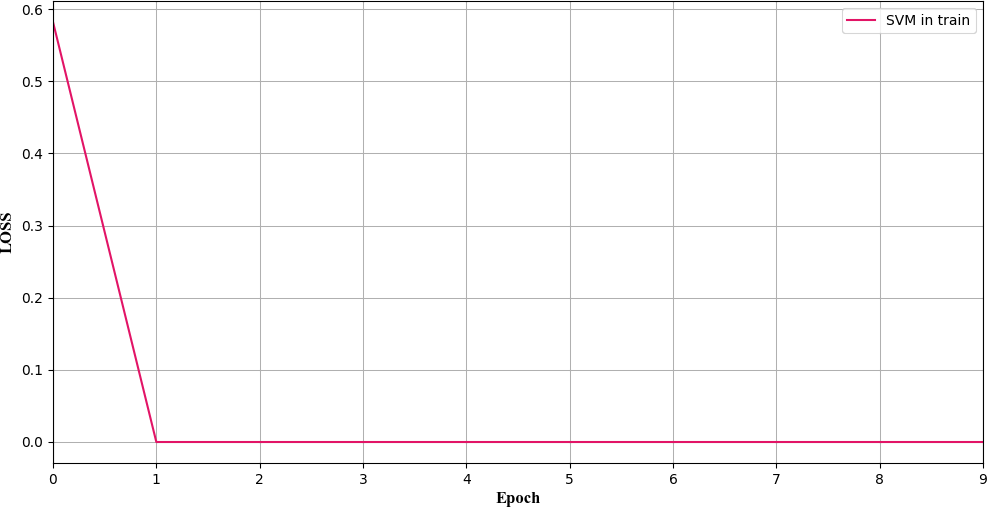
\includegraphics[width=1.0\linewidth]{exp_log/train440_valid024/LOSS_train}
    \caption[loss_train]{Loss Line Figure of All Epoch in Train Process}
    \label{fig:loss_train}
\end{figure}

\begin{figure}[h]
    \centering
    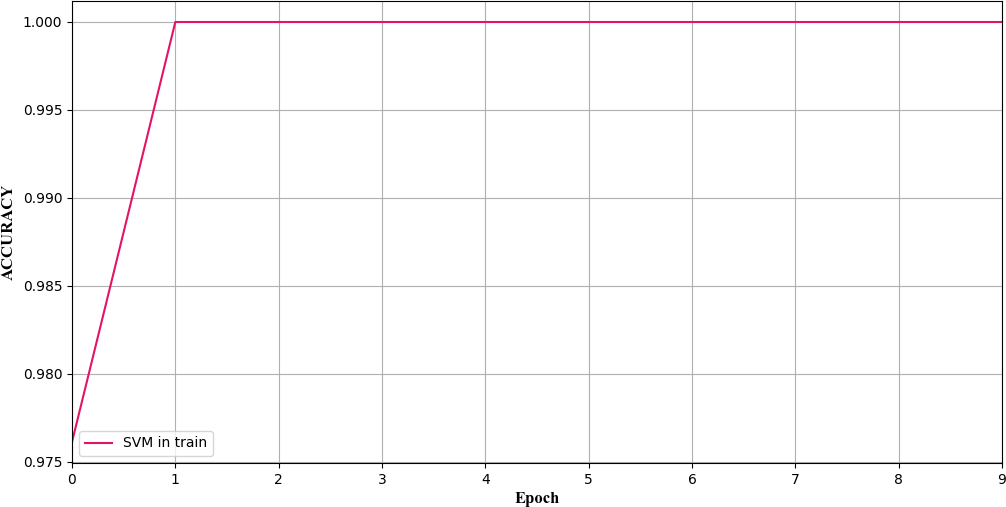
\includegraphics[width=1.0\linewidth]{exp_log/train440_valid024/ACCURACY_train}
    \caption[acc_train]{Accuracy Line Figure of All Epoch in Train Process}
    \label{fig:acc_train}
\end{figure}

为了增强模型的泛化能力并缓解过拟合问题,我们采用L2正则化,权重衰减(weight decay)参数设置为0.001。实验过程中记录了多个训练周期的数据,包括损失值、正确分类的样本数、样本总数以及分类准确率。如图\ref{fig:loss_train}所示,其中横坐标表示训练周期,纵坐标表示分类准确率为损失值。
图\ref{fig:acc_train}和图\ref{fig:acc_test}的纵坐标表示分类准确率,分别是SVM在训练和测试集上的准确率。
值得注意的是,在第一个训练周期结束后,准确率已达到相当高的水平,这表明训练数据充足,且SVM仅经过一个周期的训练即能胜任该数据集上的分类任务。

\begin{figure}[h]
    \centering
    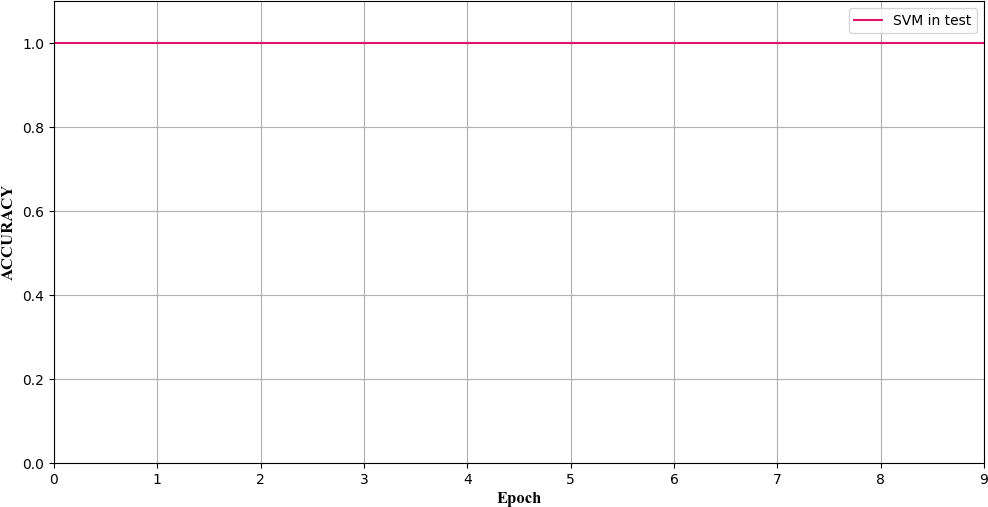
\includegraphics[width=1.0\linewidth]{exp_log/train440_valid024/ACCURACY_test}
    \caption[acc_test]{Accuracy Line Figure of All Epoch in Test Process}
    \label{fig:acc_test}
\end{figure}

为了详细展示SVM在第一周期的优化情况,我们制作了图\ref{fig:acc_train_e0},横坐标为训练的批次(batch)数,纵坐标为SVM经过之前批次的梯度下降训练后的准确率。实验结果显示,SVM分类器在初期训练阶段的准确率为50\%。
经过一个完整周期的训练后,模型在测试集上的分类准确率达到了100\%。这也可能是训练数据集规模较小的原因。

\begin{figure}[h]
    \centering
    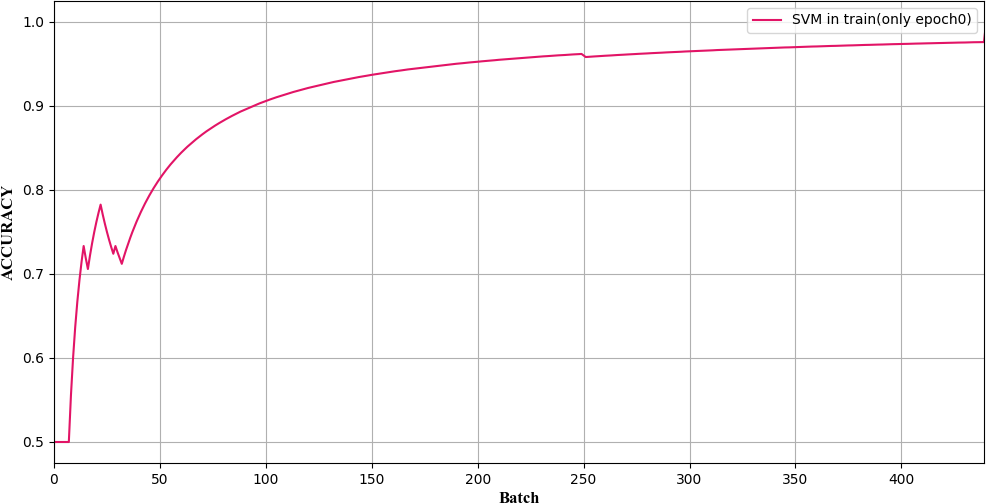
\includegraphics[width=1.0\linewidth]{exp_log/train440_valid024/ACCURACY_train_epoch0}
    \caption[acc_train_e0]{Accuracy Line Figure in Epoch 0 in Train Process}
    \label{fig:acc_train_e0}
\end{figure}

\section{Conclusion}
本研究深入探讨了支持向量机(SVM)的发展历史、技术原理及其实际应用,并在医学图像分类任务中进行了实证研究。实验结果表明,使用本研究中的数据集对SVM进行训练和测试,不仅能够有效完成相应的分类任务,而且还能取得优秀的分类性能。

\section*{Acknowledage}
谨此对National Cancer Institute Cancer Image Program表示诚挚的谢意。该机构慷慨地在互联网上公开并授权使用其高质量医疗图像数据集,为本研究的顺利开展提供了不可或缺的资源支持。

\bibliographystyle{unsrt}
\bibliography{svm}

\end{document}
